\documentclass{eplDoc}
\usepackage{placeins}


\newcommand{\docType}	{Assignment 2 : Text Categorization}
\newcommand{\docDate}	{29/03/2012}
\newcommand{\docAuthor}	{gr10 : Mulders Corentin, Pelsser Francois}
\newcommand{\courseCode}{LINGI2263}
\newcommand{\courseName}{Computational linguistics}
\usepackage{syntax}
\begin{document}
\maketitle
\newpage
\addtocounter{section}{1}

\section{Preprocessing}
To tokenize the files we had to determine where to split the sentences in words and wich types of expressions should be replaced by a token representing the type. \\ 
For slitting the tokens we simply used the whitespace as a separator as well as special characters that we didn't include in our types definitions. With the exception of the special characters "-" and "'" wich can appear inside some tokens that we didn't wish to split. \\ 
We also added markers for start and end of sentences. The start of sentences where placed before capitalized words followed by any sequence of tokens finishing by a dot or a newline. The end of sentences where then placed after any dot followed by either a start of sentence, a newline or the end of the string.
\subsection{Mapping expressions to types}
We replaced some types of expressions by aliases : 
\begin{description}
	\item[email] replaces any email
	\item[date] replaces the dates
	\item[kikoo] replaces words such as "xoXOxo" or any variation.
	\item[smiley] replaces any smiley
	\item[math] replaces mathematical expressions
	\item[punctuationfreak] replaces multiple punctuation marks.
	\item[repeatedchars] replaces any word containing a letter repeated 3 or more times in a row.
	\item[weirdcaps] replaces words with a least a non capitalized character followed by a capitalized one.
\end{description}

We also replaced occurences of "'s" by "is" and of "'m" by "am". However for the negations such as in "don't" we decided to keep the "'t" attached to "don" instead of replacing it all by "do not".
\subsection{Most frequent tokens}
After tokenizing the corpus (composed of the training files for both male and female blogs) the total number of tokens retrieved in the lexicon is  52505  distinct tokens.  \\ 
Here are the top 20 most frequent tokens types extracted from the corpus. We removed the markers <s> and </s> used to represent respectively the beginning and the end of a sentence from this top list. They were in the top 2 postiions and weren't really interesting. \\ 
\begin{center}
		\begin{tabular}{|l|c|}
			\hline
			token & frenquency \\
			\hline
			the  &  34631 \\ 
			to  &  22906 \\ 
			and  &  21281 \\ 
			a  &  19722 \\ 
			of  &  18168 \\ 
			I  &  16620 \\ 
			is  &  16436 \\ 
			in  &  11903 \\ 
			that  &  9428 \\ 
			for  &  7512 \\ 
			it  &  7179 \\ 
			on  &  6184 \\ 
			my  &  5854 \\ 
			was  &  5843 \\ 
			with  &  5705 \\ 
			you  &  5656 \\ 
			have  &  4692 \\ 
			this  &  4468 \\ 
			be  &  4186 \\ 
			as  &  4157 \\ 
			\hline
		\end{tabular}
\end{center}
 \ \\ 
We can see that the word "the" is the most frequent one as expected. 

\section{Word and N-gram counts}
Here is the graph of the number of unigrams, bigrams and trigrams for each frequency :
\FloatBarrier
\begin{figure}%
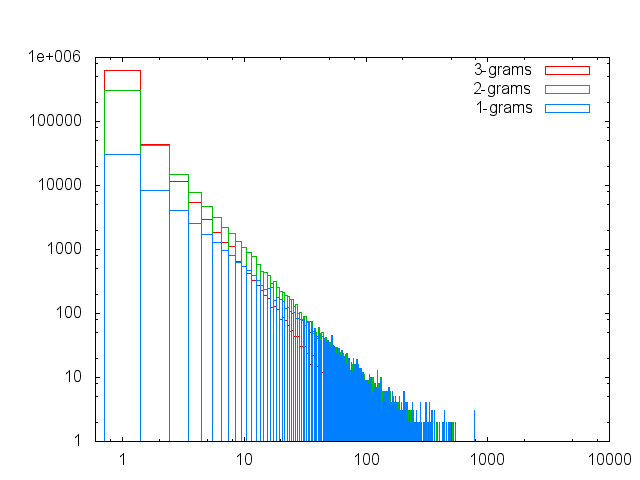
\includegraphics[width=\columnwidth]{ngramsplot.png}%
\caption{}%
\label{}%
\end{figure}
\FloatBarrier

We can see the unigrams histogram in blue and it is linear in log-log scale so Zipf's law is respected. \\ 
The same seems to be true for bigrams and trigrams. 

\section{N-gram estimation}

We computed the mean perplexity over each test set using each training set for n-grams with $n \in [1,5]$ and with the basic laplace add one smoothing and the linear interpolation smoothing. \\ 
We didn't manage to keep the consistency for the laplace model so the associated perplexities are a little bit crazy... 
\subsection{1-gram with laplace smoothing : }
\begin{tabular}{|r|c|c|c|c|} 
\hline 
	& \multicolumn{2}{c|}{On female test set} & \multicolumn{2}{c|}{On male test set}\\
training set & mean perplexity & mean perplexity OOV rate & mean perplexity & mean perplexity OOV rate \\ 
\hline 
female & 140.07300098438208 & 0.03219323101098795 & 165.55490835053433 & 0.03644707958261017\\ 
male & 134.49432287066887 & 0.03219323101098795 & 143.43047078221815 & 0.03644707958261017 \\ 
\hline 
\end{tabular} 


\subsection{1-gram with linear smoothing : }
\begin{tabular}{|r|c|c|c|c|} 
\hline 
	& \multicolumn{2}{c|}{On female test set} & \multicolumn{2}{c|}{On male test set}\\
training set	& mean perplexity & mean perplexity OOV rate & mean perplexity & mean perplexity OOV rate \\ 
\hline 
female & 1181.4392640498015 & 0.03219323101098795 & 1396.3652360335718 & 0.03644707958261017\\ 
male & 1273.3247776421954 & 0.03219323101098795 & 1357.9277431026294 & 0.03644707958261017\\ 
\hline 
\end{tabular} 

\subsection{2-gram with laplace smoothing : }
\begin{tabular}{|r|c|c|c|c|} 
\hline 
& \multicolumn{2}{c|}{On female test set} & \multicolumn{2}{c|}{On male test set}\\
training set & mean perplexity & mean perplexity OOV rate & mean perplexity & mean perplexity OOV rate \\ 
\hline 
female & 6597.051090993472 & 0.03219323101098795 & 7526.464184988605 & 0.03644707958261017\\ 
male & 6751.450681527784 & 0.03219323101098795 & 7068.504328026753 & 0.03644707958261017\\ 
\hline 
\end{tabular} 


\subsection{2-gram with linear smoothing : }
\begin{tabular}{|r|c|c|c|c|} 
\hline 
& \multicolumn{2}{c|}{On female test set} & \multicolumn{2}{c|}{On male test set}\\
training set & mean perplexity & mean perplexity OOV rate & mean perplexity & mean perplexity OOV rate \\ 
\hline 
female & 85.85618860497664 & 0.03219323101098795 & 98.29094897820075 & 0.03644707958261017\\ 
male & 94.7289894781771 & 0.03219323101098795 & 93.48257298944773 & 0.03644707958261017\\ 
\hline 
\end{tabular} 
\subsection{3-gram with laplace smoothing : }
\begin{tabular}{|r|c|c|c|c|} 
\hline 
& \multicolumn{2}{c|}{On female test set} & \multicolumn{2}{c|}{On male test set}\\
training set & mean perplexity & mean perplexity OOV rate & mean perplexity & mean perplexity OOV rate \\ 
\hline 
female & 19419.704289536854 & 0.03219323101098795 & 21080.08273975077 & 0.03644707958261017\\ 
male & 19857.104934164177 & 0.03219323101098795 & 20674.655403927376 & 0.03644707958261017\\ 
\hline 
\end{tabular} 

\subsection{3-gram with linear smoothing : }
\begin{tabular}{|r|c|c|c|c|} 
\hline 
& \multicolumn{2}{c|}{On female test set} & \multicolumn{2}{c|}{On male test set}\\
training set & mean perplexity & mean perplexity OOV rate & mean perplexity & mean perplexity OOV rate \\ 
\hline 
female & 74.05775785805339 & 0.03219323101098795 & 96.82676770775483 & 0.03644707958261017\\ 
male & 87.29893378787449 & 0.03219323101098795 & 88.4301357336149 & 0.03644707958261017\\ 
\hline 
\end{tabular} 

\subsection{4-gram with laplace smoothing : }
\begin{tabular}{|r|c|c|c|c|} 
\hline 
& \multicolumn{2}{c|}{On female test set} & \multicolumn{2}{c|}{On male test set}\\
training set & mean perplexity & mean perplexity OOV rate & mean perplexity & mean perplexity OOV rate \\ 
\hline 
female & 23270.25113767307 & 0.03219323101098795 & 24783.006381785264 & 0.03644707958261017\\ 
male & 23512.386931883306 & 0.03219323101098795 & 24376.779729652386 & 0.03644707958261017\\ 
\hline 
\end{tabular} 

\subsection{4-gram with linear smoothing : }
\begin{tabular}{|r|c|c|c|c|}  
\hline 
& \multicolumn{2}{c|}{On female test set} & \multicolumn{2}{c|}{On male test set}\\
training set & mean perplexity & mean perplexity OOV rate & mean perplexity & mean perplexity OOV rate \\ 
\hline 
female & 132.88670099907827 & 0.03219323101098795 & 174.63117442256916 & 0.03644707958261017 \\ 
male & 151.2064322011711 & 0.03219323101098795 & 153.94702577858564 & 0.03644707958261017\\ 
\hline 
\end{tabular} 

\subsection{5-gram with laplace smoothing : }
\begin{tabular}{|r|c|c|c|c|} 
\hline 
& \multicolumn{2}{c|}{On female test set} & \multicolumn{2}{c|}{On male test set}\\
training set & mean perplexity & mean perplexity OOV rate & mean perplexity & mean perplexity OOV rate \\ 
\hline 
female & 23428.567965680333 & 0.03219323101098795 & 24823.951627660903 & 0.03644707958261017\\ 
male & 23588.180660734663 & 0.03219323101098795 & 24415.93450835315 & 0.03644707958261017\\ 
\hline 
\end{tabular} 
\subsection{5-gram with linear smoothing : }
\begin{tabular}{|r|c|c|c|c|} 
\hline 
& \multicolumn{2}{c|}{On female test set} & \multicolumn{2}{c|}{On male test set}\\
training set & mean perplexity & mean perplexity OOV rate & mean perplexity & mean perplexity OOV rate \\ 
\hline 
female & 164.70561612766298 & 0.03219323101098795 & 214.29336077008773 & 0.03644707958261017\\ 
male & 190.28328162528635 & 0.03219323101098795 & 193.30692013526775 & 0.03644707958261017\\ 
\hline 
\end{tabular} 

\subsection{Conclusions from the perplexities}

We notice that most of the time the perplexity islower on the same test set as the training set used. This is expected since sets from the same gender match better. \\ \\ 
We also notice that the lowest perplexity is for linear smoothing with 3-grams. We'll see later if this reflects on the quality of the prediction.

\section{Categorization of blog messages per gender}

Here are the confuction matrices that we obtained with unigrams, trigrams and pentagrams while using laplace add one smoothing and linear interpolation smoothing. Each line corresponds to the results obtained for the lines of a given test set. Columns represent the value guessed. 
\subsection{1-grams with laplace smoothing :} 
\begin{tabular}{|r|c|c|} 
\hline 
 & male & female \\ 
\hline 
male & 596 & 78 \\ 
female & 342 & 205 \\ 
\hline 
\end{tabular} 
\subsection{1-grams with linear smoothing :} 
\begin{tabular}{|r|c|c|} 
\hline 
 & male & female \\ 
\hline 
male & 326 & 348 \\ 
female & 93 & 454 \\ 
\hline 
\end{tabular} 
\subsection{3-grams with laplace smoothing :} 
\begin{tabular}{|r|c|c|} 
\hline 
 & male & female \\ 
\hline 
male & 382 & 292 \\ 
female & 151 & 396 \\ 
\hline 
\end{tabular} 
\subsection{3-grams with linear smoothing :} 
\begin{tabular}{|r|c|c|} 
\hline 
 & male & female \\ 
\hline 
male & 402 & 272 \\ 
female & 148 & 399 \\ 
\hline 
\end{tabular} 
\subsection{5-grams with laplace smoothing :} 
\begin{tabular}{|r|c|c|} 
\hline 
 & male & female \\ 
\hline 
male & 411 & 263 \\ 
female & 198 & 349 \\ 
\hline 
\end{tabular} 
\subsection{5-grams with linear smoothing :} 
\begin{tabular}{|r|c|c|} 
\hline 
 & male & female \\ 
\hline 
male & 399 & 275 \\ 
female & 164 & 383 \\ 
\hline 
\end{tabular} 

\subsection{Conclusions}
\subsubsection{Optimal model order and smoothing technique} 

First of all we can easilty tell that the linear interpolation smoothing tends to be better than the laplace add one. For unigrams laplace results on detecting female test samples are disastrous. \\ 
Then about the optimal order, unigrams be be excluded since the results are pretty random. However with linear smoothing the results with 3-grams and 5-grams are nearly the sames. But since 5-grams require more computation power the 3-grams can be selected as optimal. 
 

\subsubsection{Correlation to the perplexity results}

We noted that the lowest perplexities were obtained with 3-grams linear smoothing. This is also the model order and smoothing technique that we selected as optimal from the confusion matrices so the perplexity results were a good indicator of the classification accuracy. 

\end{document}
